\newcommand{\study}[1]{
\newif\ifhiggs

\IfFileExists{abc.tex}{\higgstrue}{\higgsfalse}
\ifhiggs
  \loop
  \begin{frame}
  \repeat
\fi
}
% if 
\newcommand{\widP}{2.4in}
\newcommand{\widF}{2.4in}
\newcommand{\simu}{one}
% RUN NEW CONTROL SIMS
\newcommand{\polycube}{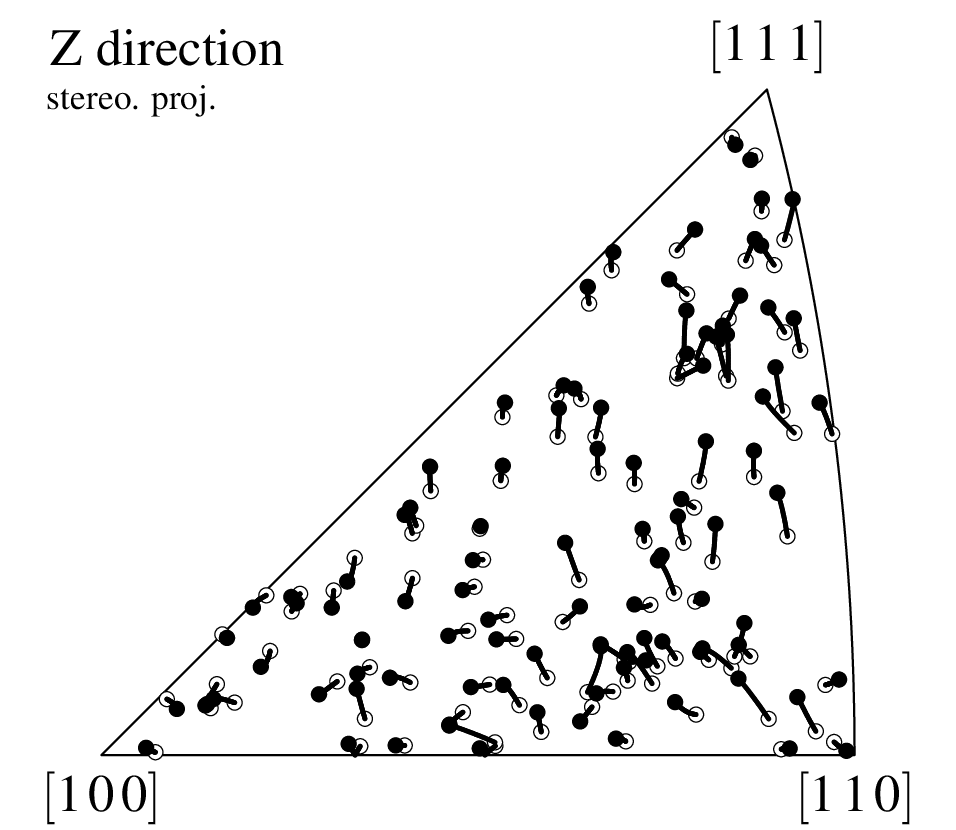
\includegraphics[width=\widP]{figures/cubic_domain_control.png}}
\newcommand{\polyelongated}{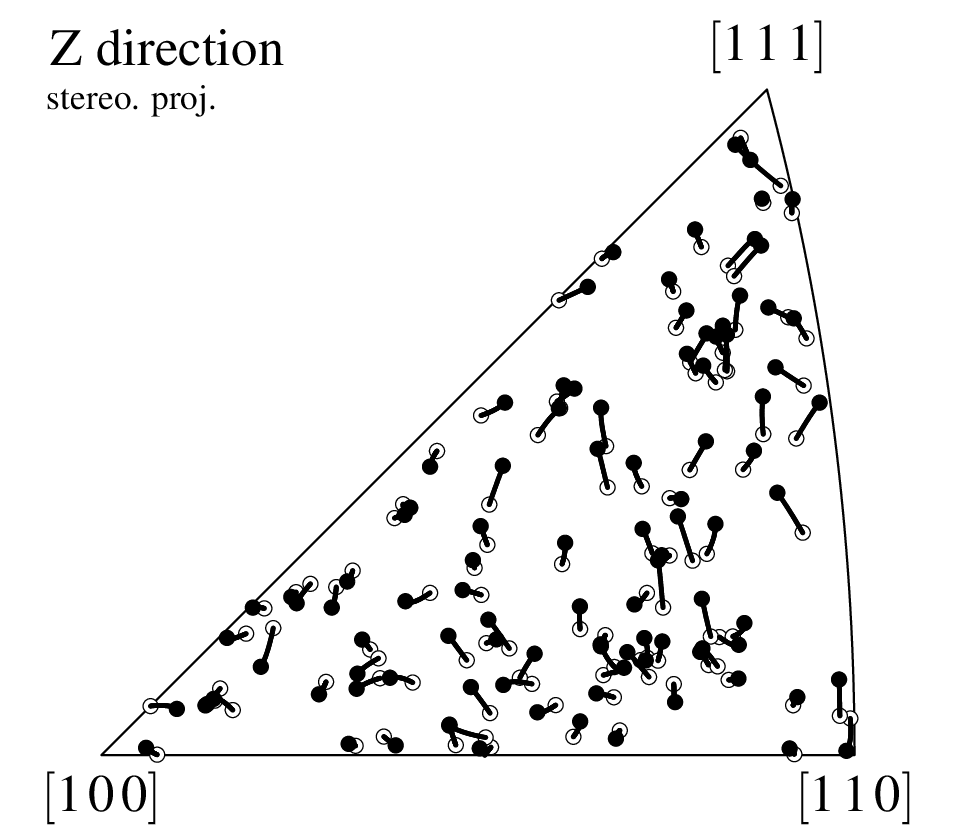
\includegraphics[width=\widP]{figures/elongated_domain_control.png}}
%
\newcommand{\cTimesOTF}[2]{\includegraphics[width=\widF]{figures/Cube_125_#1ss_set_#2.png}}
\newcommand{\cTimesOFO}[2]{\includegraphics[width=\widF]{figures/Cube_150_#1ss_set_#2.png}}
\newcommand{\cTimesOSF}[2]{\includegraphics[width=\widF]{figures/Cube_175_#1ss_set_#2.png}}
\newcommand{\cTimesTH }[2]{\includegraphics[width=\widF]{figures/Cube_200_#1ss_set_#2.png}}
\newcommand{\cTimesFH }[2]{\includegraphics[width=\widF]{figures/Cube_400_#1ss_set_#2.png}}
%
\newcommand{\eTimesOTF}[2]{\includegraphics[width=\widF]{figures/Elongated_125_#1ss_set_#2.png}}
\newcommand{\eTimesOFO}[2]{\includegraphics[width=\widF]{figures/Elongated_150_#1ss_set_#2.png}}
\newcommand{\eTimesOSF}[2]{\includegraphics[width=\widF]{figures/Elongated_175_#1ss_set_#2.png}}
\newcommand{\eTimesTH }[2]{\includegraphics[width=\widF]{figures/Elongated_200_#1ss_set_#2.png}}
\newcommand{\eTimesFH }[2]{\includegraphics[width=\widF]{figures/Elongated_400_#1ss_set_#2.png}}
%
\newcommand{\tablee}[1]{ 
\footnotesize{
    \begin{tabular}{|c|c|c|c|c|c|c|c|c|c|c|c|c|}
        \hline
        Simulation &$\hkl(0 1 -1)$ $\hkl[1 1 1]$   &$\hkl(1 0 -1)$ $\hkl[1 1 1]$   &$\hkl(1 -1 0)$ $\hkl[1 1 1]$   &$\hkl(0 1 1)$  $\hkl[1 1 -1]$  &$\hkl(1 0 1)$  $\hkl[1 1 -1]$  &$\hkl(1 -1 0)$ $\hkl[1 1 -1]$  &$\hkl(0 1 1)$  $\hkl[1 -1 1]$  & $\hkl(1 0 -1)$ $\hkl[1 -1 1]$  &$\hkl(1 1 0)$  $\hkl[1 -1 1]$  &$\hkl(0 1 -1)$ $\hkl[1 -1 -1]$ &$\hkl(1 0 1)$  $\hkl[1 -1 -1]$ &$\hkl(1 0 1)$  $\hkl[1 -1 -1]$ \\ \hline \hline
        %\hline
        %&0&1&2&3&4&5&6&7&8&9&10&11\\
         Strength #    & 39.0    & 39.0    & 39.0    & 39.0& 39.0   & 39.0     & 39.0    & 39.     0& 39.0     & 39.0   & 39.0    & 39.0    \\ \hline             
    \end{tabular}}
}
%
\newcommand{\simulation}[3]{
\begin{frame}{Simset number #3: #1 slip systems altered set #2}
    \begin{table}[]
        \centering
        \begin{tabular}{|c|ccccc|} 
        \hline
        Isotropic & 125\% & 150\% & 175\% & 200\% & 400\% &
        \hline
             \polycube&      \cTimesOTF{#1}{#2}& \cTimesOFO{#1}{#2}& \cTimesOSF{#1}{#2}& \cTimesTH{#1}{#2}& \cTimesFH{#1}{#2} \\
             \hline
             \polyelongated& \eTimesOTF{#1}{#2}& \eTimesOFO{#1}{#2}& \eTimesOSF{#1}{#2}& \eTimesTH{#1}{#2}& \eTimesFH{#1}{#2}\\
            \hline
        \end{tabular}
    \end{table}
    %\tablee{#3}
\end{frame}
\begin{frame}{Compiled trajectories: #1 slip systems altered set #2}
    \begin{columns}
        \begin{column}{0.4\textwidth}
            \begin{block}{Cubic domain:}
            \hspace{1in}
                \includegraphics[width=\textwidth]{figures/Cube_set_#2_#1ss.png}
            \end{block}
        \end{column}
        %
        
        %
        \begin{column}{0.4\textwidth}
            \begin{block}{Elongated domain:}
            \hspace{1in}
                \includegraphics[width=\textwidth]{figures/Elongated_set_#2_#1ss.png}
            \end{block}
        \end{column}
    \end{columns}
\end{frame}
}
\simulation{2}{1}{001-005}
\simulation{2}{2}{006-010}
\simulation{2}{3}{011-015}
\simulation{2}{4}{016-020}
\simulation{2}{5}{021-025}

\simulation{4}{1}{026-030}
\simulation{4}{2}{031-035}
\simulation{4}{3}{036-040}
\simulation{4}{4}{041-045}
\simulation{4}{5}{046-050}

\simulation{6}{1}{051-055}
\simulation{6}{2}{056-060}
\simulation{6}{3}{061-065}
\simulation{6}{4}{066-070}
\simulation{6}{5}{071-075}